% Tikz File 'model640.tex'
\documentclass{standalone}

\usepackage{tikz} %Graphics
\usetikzlibrary{shapes.geometric, arrows}
\tikzstyle{title} = [text centered]
\tikzstyle{block} = [rectangle, rounded corners, minimum width=3cm, minimum height=1cm,text centered, draw=black, fill=blue!30]
\tikzstyle{conv} = [rectangle, rounded corners, minimum width=3cm, minimum height=1cm,text centered, draw=black, fill=blue!30]
\tikzstyle{batchnorm} = [rectangle, rounded corners, minimum width=3cm, minimum height=1cm,text centered, draw=black, fill=blue!30]
\tikzstyle{relu} = [rectangle, rounded corners, minimum width=3cm, minimum height=1cm,text centered, draw=black, fill=orange!30]
\tikzstyle{maxpool} = [rectangle, rounded corners, minimum width=3cm, minimum height=1cm,text centered, draw=black, fill=red!30]
\tikzstyle{arrow} = [thick,->,>=stealth]

%\usetikzlibrary{...}
\begin{document}
	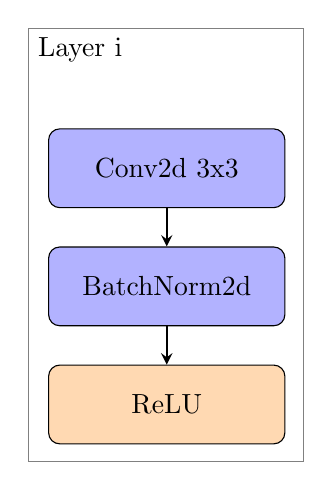
\begin{tikzpicture}[node distance=1.5cm]
				\node (decomp) [title] { Layer i };
		\draw [draw=black!50] (decomp.north west) rectangle +(3.5cm, -5.5cm);	
		\node (c1) [conv, below of = decomp, xshift=11mm] {Conv2d 3x3};
		\node (b1) [batchnorm, below of=c1] {BatchNorm2d};
		\node (r1) [relu, below of=b1] {ReLU};
		\draw [arrow] (c1) -- (b1);
		\draw [arrow] (b1) -- (r1);
	\end{tikzpicture}
\end{document}
